\section{OpenCL ray casters}
\label{sec:opencl_caster}

Before altering the existing prototype after its analysis, a separate branch in SVN has been created to allow experimenting with the existing code without disturbing the other members of the team. Before development could be started, further tools had to be installed. As the GPU provided by RISC was from NVIDIA, NVIDIA's CUDA Toolkit (version 5.0) was installed which contains the required OpenCL header files and libraries. Furthermore, the OpenCL C++ wrapper provided by Khronos (cl.hpp) was downloaded from their website. Several weeks later, also Intel's SDK for OpenCL Applications 2013 was added, which provided a limited OpenCL debugger some smaller extensions to Visual Studio. Then, a separate project was added to the existing Visual Studio solution and the necessary include and library paths configured in order to use OpenCL.

\subsection{OpenCL ray casting driver}

Implementing a ray caster with OpenCL started by designing a small infrastructure which should fulfill some requirements:

\begin{itemize}
	\item Only one class should be needed by \lstinline!DebugView! (the main application class) in order to communicate with the OpenCL ray caster.
	\item As the OpenCL ray casters will be developed incrementally and several different ideas exists, it should be possible to write multiple, interchangeable casters.
	\item It should be possible to reload an OpenCL caster at run time. As loading larger scenes may take up to some minutes and the OpenCL source code is read in and compiled at run time, this feature allows it to change the OpenCL source code of a caster at run time and reload it without having to relaunch the host application.
	\item Several options should be adjustable by the main application via the console (which may trigger a recompilation of the kernels or a reconfiguration of the OpenCL environment).
	\item If a ray caster crashes or OpenCL experiences any problems, it should be possible to relaunch the complete OpenCL environment without having to restart the whole application. 
\end{itemize}

Derived from these requirements, a simple architecture has been designed which is shown in the simplified class diagram in figure \ref{fig:enlight_opencl_class_diagram}.

\begin{figure}
\centering
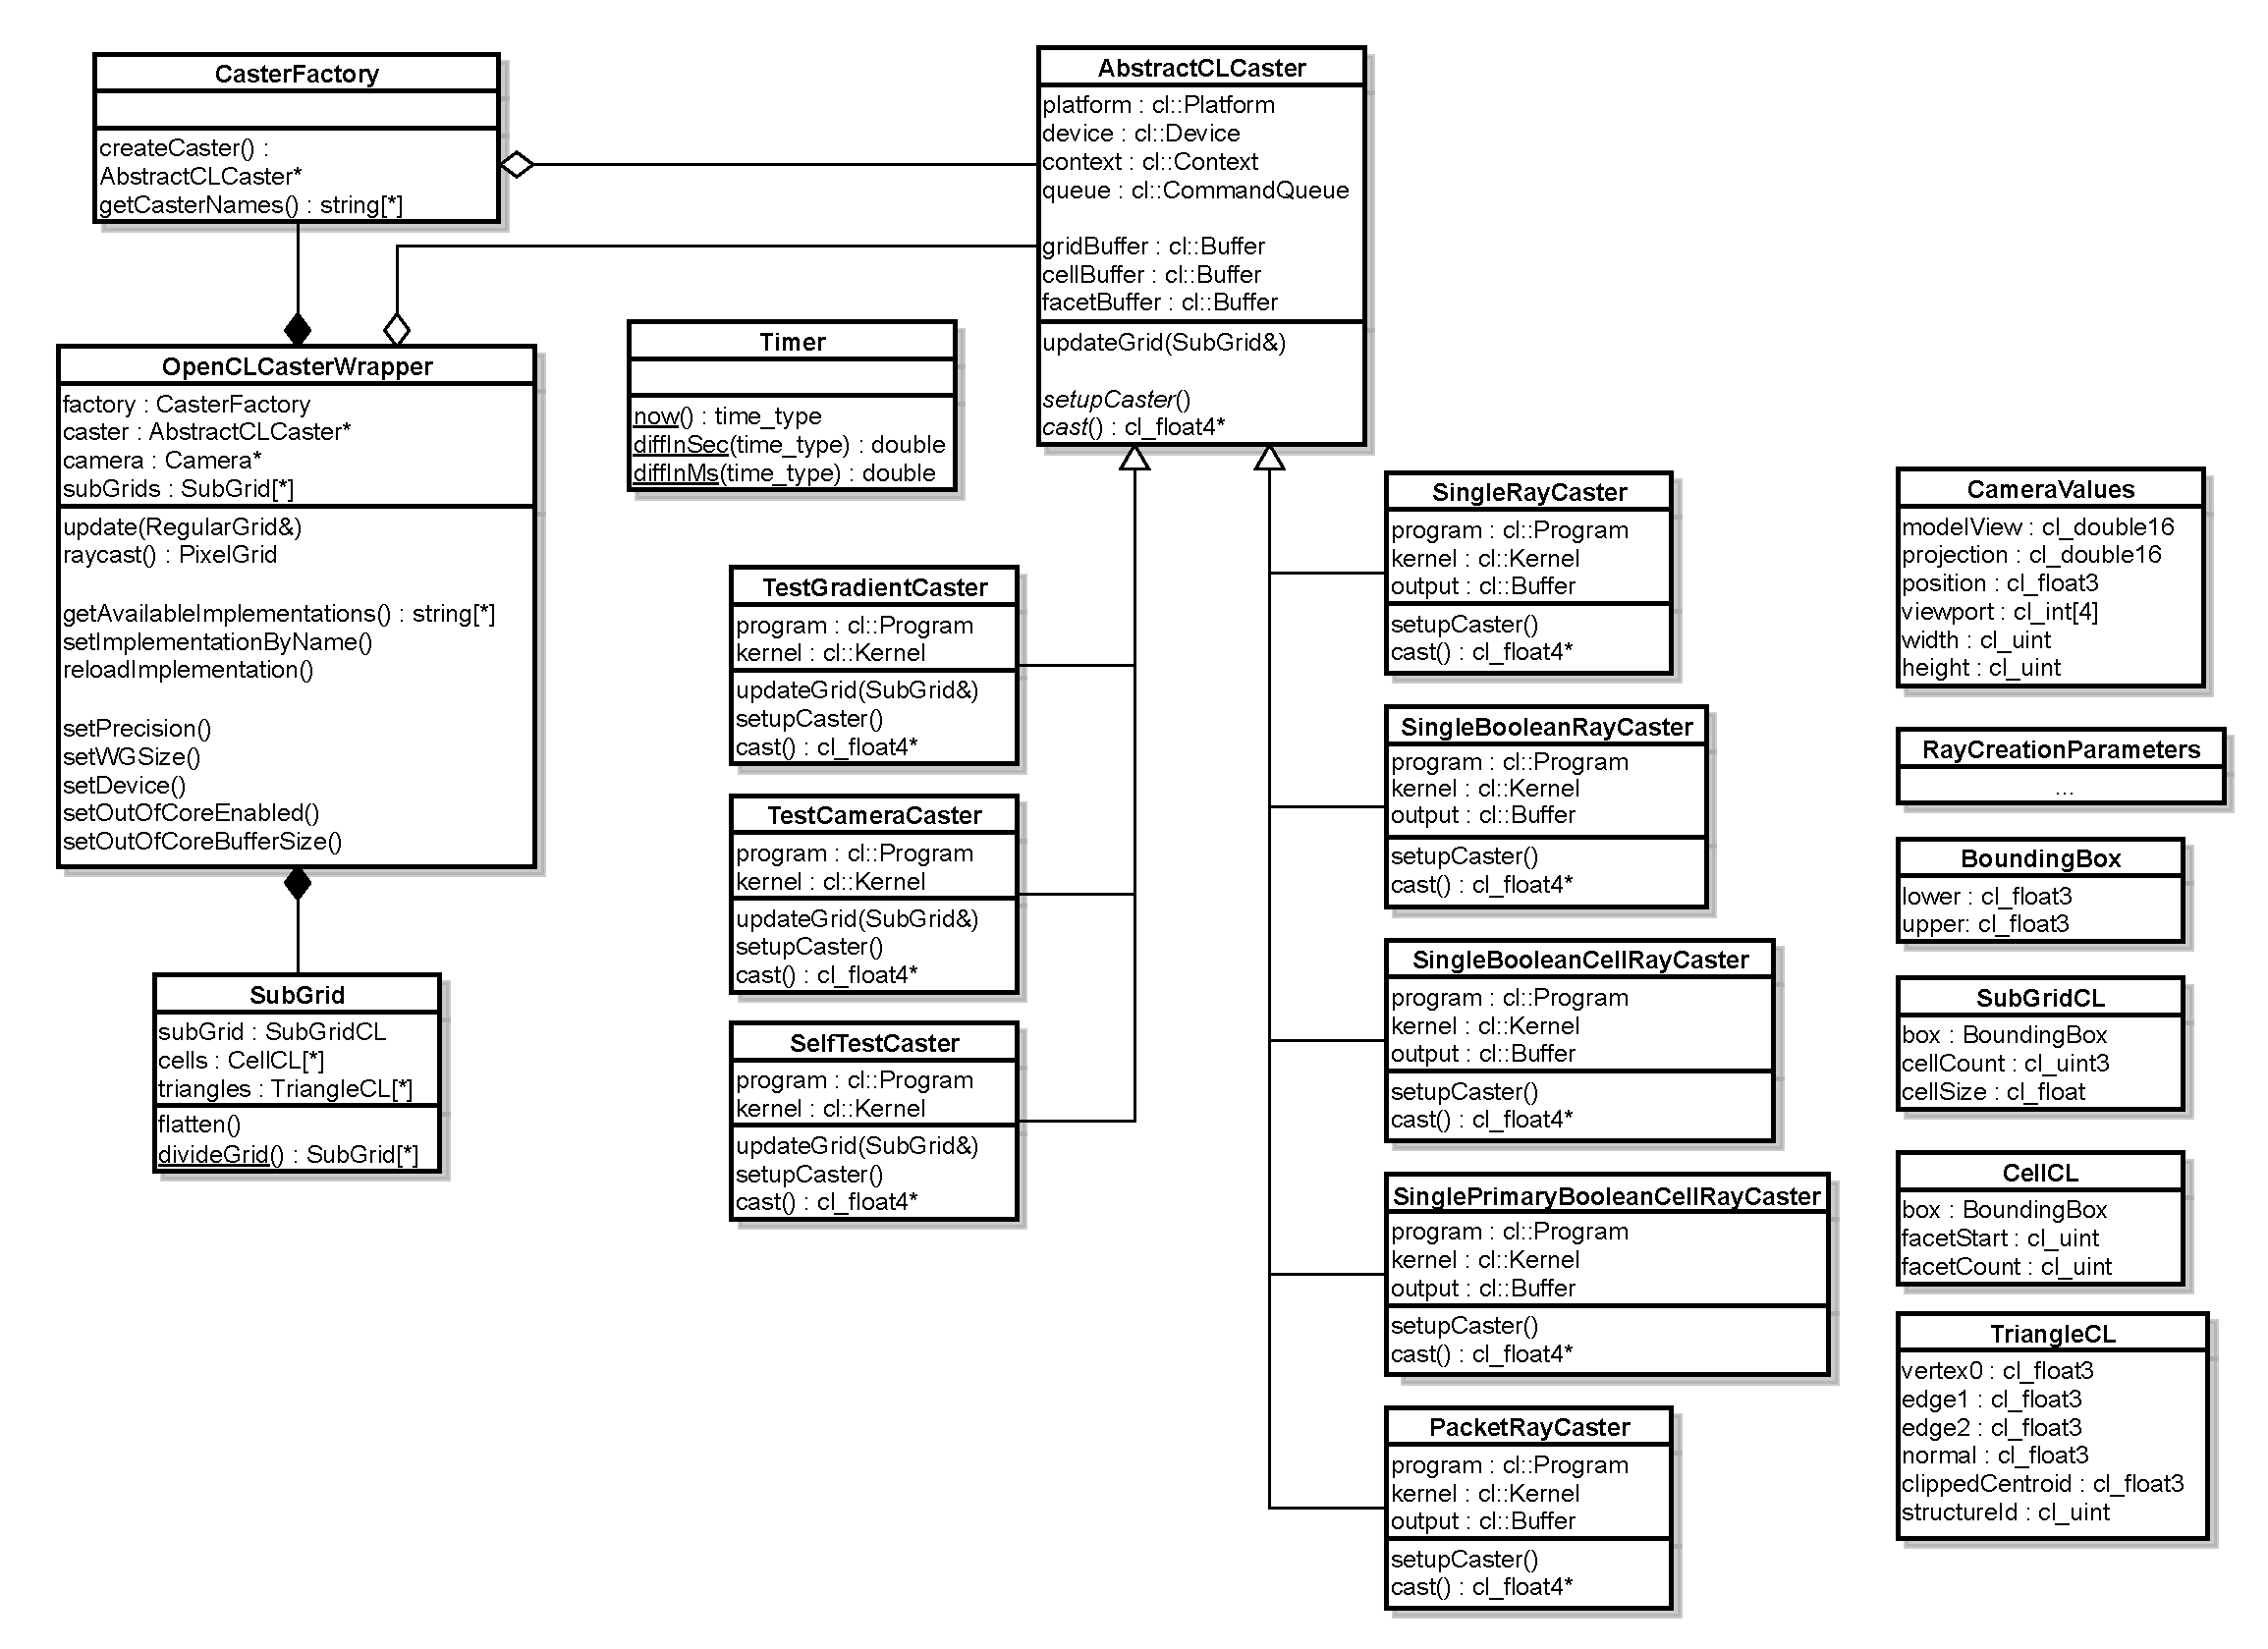
\includegraphics[width=\textwidth]{enlight_opencl_class_diagram}
\caption{Simplified class diagram of the OpenCL ray casting driver.}
\label{fig:enlight_opencl_class_diagram}
\end{figure}

The central class and entry point of the OpenCL ray casting environment is the \lstinline!OpenCLCasterWrapper! class. An instance of this class is maintained by \lstinline!DebugView!, similar to the \lstinline!RayCasterWrapper! (cf. figure \ref{fig:enlight_class_diagram}). The \lstinline!OpenCLCasterWrapper! offers several methods for interacting with an OpenCL caster. Most importantly, it offers an \lstinline!update! method taking a reference to the \lstinline!RegularGrid! maintained by the main application which holds all relevant data of the scene. This method has to be called at least once before ray casting can be done. The \lstinline!raycast! method performs the main work of generating an image. The created image with depth information is also stored inside an object of \lstinline!PixelGrid! and passed back to the main application. \\
For managing the underlying ray casting implementations, each caster is assigned a name. This assignment is managed by the \lstinline!CasterFactory!, which is used by the \lstinline!OpenCLCasterWrapper! to provide a list of available implementations and to allow selection and creation of casters by their name. The currently loaded caster is pointed to by the \lstinline!caster! member of the \lstinline!OpenCLCasterWrapper!. Furthermore, a reload method is provided for recreating the currently loaded caster. \\
Additionally, several options concerning OpenCL and the implemented ray casters may be set by the main application using the console. The \lstinline!OpenCLCasterWrapper! offers further methods for configuring several values such as the used floating point precision, work group size, OpenCL platform and device as well as enabling out of core casting and adjusting the out of core buffer size (cf. chapter \ref{sec:out_of_core}).

The \lstinline!SubGrid! class is responsible for holding the full or a part of the grid. and for transforming the grid's representation into buffers which can be pushed to the GPU. Details to both usages will be discussed with the caster implementations requiring this functionality.

The \lstinline!Timer! class is a small helper class for measuring durations. It is used to print to the time required for certain operations inside the driver such as ray casting a frame, compiling a kernel or ray casting an out of core mesh in multiple passes.

The second most important class is \lstinline!AbstractCLCaster!. It is the base of all ray caster classes and is responsible for setting up the OpenCL environment for each caster. Every ray caster implementation has to inherit from this class and must implement the both pure virtual functions \lstinline!setupCaster! and \lstinline!cast!. While \lstinline!cast! is called directly from the \lstinline!OpenCLCasterWrapper!, \lstinline!setupCaster! is a template method inside \lstinline!AbstractCLCaster! and is called during the casters construction, after OpenCL has been initialized. The derived caster implementation should create its kernels and further resources here. The \lstinline!updateGrid! method is already implemented in the base class, as it works equally for all ray casting implementations which require the grid on the GPU (all non-test casters). Furthermore, \lstinline!AbstractCLCaster! offers a variety of utility methods which can be used by derived casters.

On the right side of the class diagram (figure \ref{fig:enlight_opencl_class_diagram}) are several structures. \lstinline!CameraValues! is used to transport relevant camera information from the \lstinline!OpenCLCasterWrapper! into the caster implementations. This avoids dragging the \lstinline!Camera! class and its dependencies deeper into the OpenCL project (The grid is also converted into one or multiple instances of \lstinline!SubGrid! before it is passed into the caster implementations in order to reduce avoidable dependencies). The remaining structures are all used as data transfer objects between the OpenCL ray casters on the host application and the GPU. Therefore, only types defined in the corresponding OpenCL header are used (e.g. \lstinline!cl_uint!, \lstinline!cl_float3!). 


\subsection{TestGradientCaster}

The first caster is a proof of concept to test the functionality of the OpenCL environment. It does not use the grid, loaded geometries or the camera's current values. The \lstinline!TestGradientCaster! only loads the OpenCL kernel source code from a file and compiles it using corresponding helper methods from \lstinline!AbstractCLCaster! inside the overridden \lstinline!setupCaster! method. The \lstinline!updateGrid! method is also overridden but empty, as no grid buffers have to be created and uploaded. Inside the \lstinline!cast! method, an output buffer is created capable of holding a \lstinline!cl_float4! value (red, green, blue, depth) for each pixel of the requested output image (determined by the fields \lstinline!width! and \lstinline!height! of \lstinline!CameraValues!, of which an instance is passed to the \lstinline!cast! method). Then, the loaded kernel is enqueued on the command queue for execution on the GPU. The global work size of the kernel is only one dimensional and the number of output pixels rounded up to be a multiple of the maximum allowed work group size. Each kernel invocation then derives the output pixels x and y coordinate from the global id of the work item and writes a color value to the output buffer. The red channel of the color is the x coordinate divided by the output image width, the green channel is the y coordinate divided by the height and the blue and depth channel are set to zero. After the kernel has executed, the result is read back to the host into an allocated \lstinline!cl_float4! array, which is then returned by the \lstinline!cast! method. The \lstinline!OpenCLCasterWrapper! converts this array into an instance of \lstinline!PixelGrid! which is then passed back to the main application for display.

The resulting gradient of the TestGradientCaster is shown in figure \ref{fig:testgradient}.

\begin{figure}
\centering
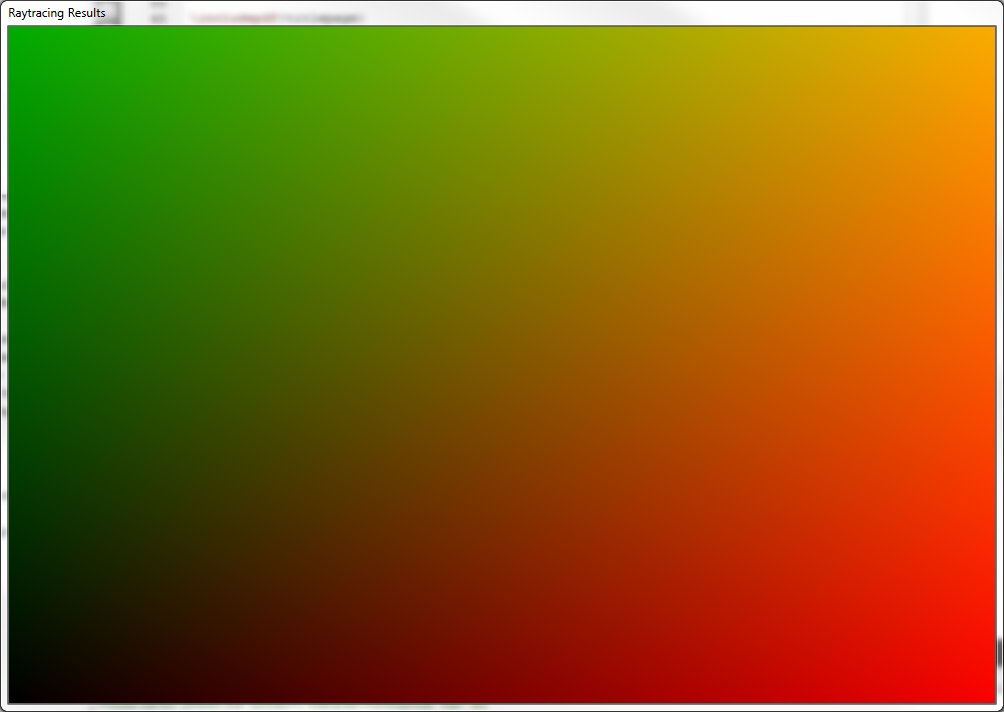
\includegraphics[width=0.5\textwidth]{testgradient}
\caption{Screenshot of the OpenCL kernel output of the TestGradientCaster.}
\label{fig:testgradient}
\end{figure}


\subsection{TestCameraCaster}

The next test caster is based on the \lstinline!TestGradientCaster!. The goal of this caster is to test the creation of rays according to the current camera settings. Therefore, the \lstinline!CameraValues! instance passed to the \lstinline!cast! method is converted into a \lstinline!RayCreationParameters! structure, which is passed as an argument to the kernel. This structure contains selected fields of the model view and projection matrix as well as several precalculated values which are used to create the ray direction vectors for a given x and y coordinate on the image plane. The kernel itself stores the vertices of 12 triangles forming a simple cube placed at the coordinate space origin in constant memory (a special part of the global memory). The kernel is enqueued with a two dimensional global work size of the output images width and height (both rounded up to be a multiple of the configured work group size). Each work item than calculates the ray direction of the ray traveling through the pixel of the work group item's x and y coordinate on the image plane. With the origin at the camera position, this ray is then intersected with the 12 triangles of the cube. The intersection routine used is an adapted version of the "Fast, Minimum Storage Ray/Triangle Intersection" (name of the paper) approach presented by Tomas Möller and Ben Trumbore. \cite{triangle_intersection}. The intersections are depth sorted to find the correct intersection point and hit triangle. A color value for the pixel is then calculated using the dot product of the ray's direction vector and the surface normal of the hit triangle. After the kernel has run, the resulting buffer is processed as by the TestGradientCaster.

%\subsubsection{Ray creation routines}
%
%ray creation parameters, matrices, formulas

%\subsubsection{Fast triangle intersection routine}
%
%paper + explanation

The resulting image of a cube which rotates synchronously with the OpenGL visualization of the loaded scene is shown in figure \ref{fig:testcamera}.

\begin{figure}
\centering
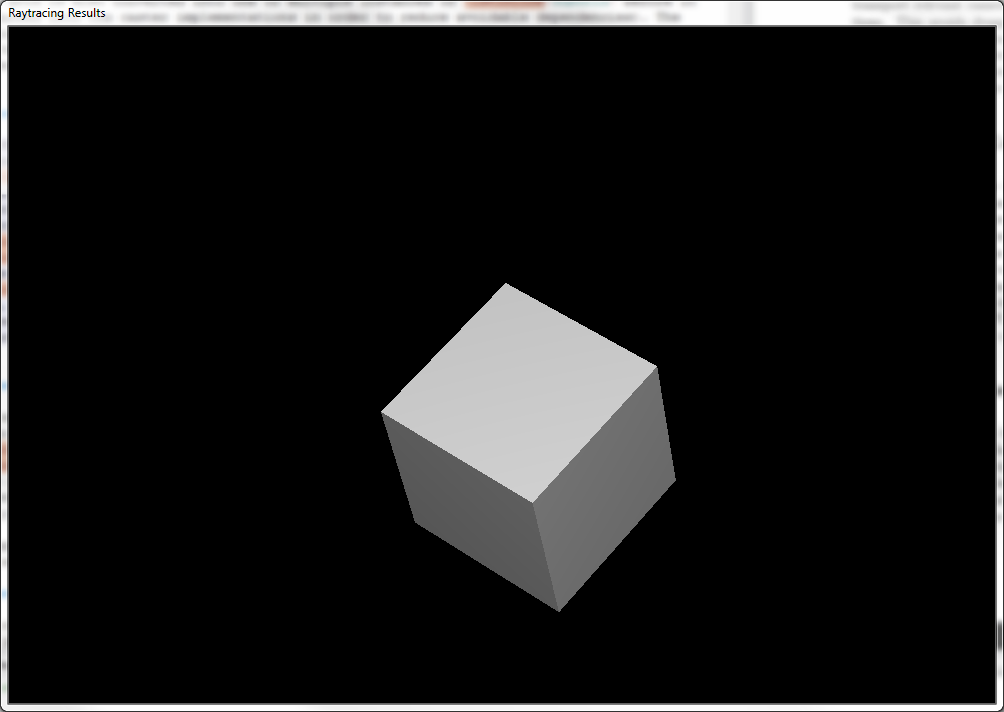
\includegraphics[width=0.5\textwidth]{testcamera}
\caption{Screenshot of the OpenCL kernel output of the TestCameraCaster.}
\label{fig:testcamera}
\end{figure}


\subsection{SelfTestCaster}

The self test caster is a simple test of the structures used in host application and OpenCL interaction. More specifically, the SelfTestCaster calculates the size of all structures used in memory transfers between the host and the GPU on the host and enqueues a kernel retrieving the corresponding values on the device side. These values are compared against each other and an error is yielded if any pair of them is not equal.
The reason why problems might occur on this level is the varying struct member alignment and padding carried out by different compilers. Although the data alignment of OpenCL is based on the one of ISO C99, some additions have to be made for OpenCL's built in vector types (cf. OpenCL specification 6.1.5 \cite{opencl_spec}). In particular, OpenCL has built in vector types which have to be aligned to a memory address being an even multiple of their size and a power of two. A \lstinline!float3! value for example, with a theoretical size of 12 bytes, is therefore aligned to a 16 byte boundary. However, the corresponding \lstinline!cl_float3! typedef on the host application (defined in cl.h) is backed by a structure containing a four element float array. This ensures that both types, \lstinline!float3! inside OpenCL and \lstinline!cl_float3! on the host application, are of equal size (16 byte), but it cannot guarantee a proper alignment as the OpenCL \lstinline!float3! type will be 16 bytes aligned and the \lstinline!cl_float3! structure (an array of floats) only to a four byte boundary. This has significant consequences if such vector types are used within structures as the size of the structs may be different (typically larger) inside an OpenCL kernel than within the host application. Consequently, enforcing proper alignment is partially up to the programmer and has to be declared for the affected structures (e.g. with \lstinline! __declspec(align(sizeof(cl_float3)))! using Intel's C++ compiler).
As the kernel does not create an output image, an empty buffer is allocated on the host and returned.


\subsection{SingleRayCaster}

The SingleRayCaster is the first full ray casting attempt. It is based on the TestCameraCaster considering the host code, the ray creation inside the work items and the triangle intersection routine. However, instead of using statically coded geometry inside the kernel, the grid containing the loaded geometries from the main application is used. Therefore, an appropriate memory layout has to be defined which fits well to the concept of OpenCL buffers. To traverse the grid, the 3D DDA algorithm presented in chapter \ref{sec:regular_grids} has to be implemented. No counting is performed and no distinction of triangles from different structures and their facing (normal vector) is made.

As the data structure holding the grid on the host application is to some degree hierarchical (grid uses dynamically allocated array of cells, cells hold arrays of pointers to facets), the first step before any transfer to the GPU can happen is to flatten the data structure into corresponding OpenCL buffers. Figure \ref{fig:buffer_layout} shows how the grid data structure can be represented using linear arrays by substituting pointers by indexes.

\begin{figure}
\centering
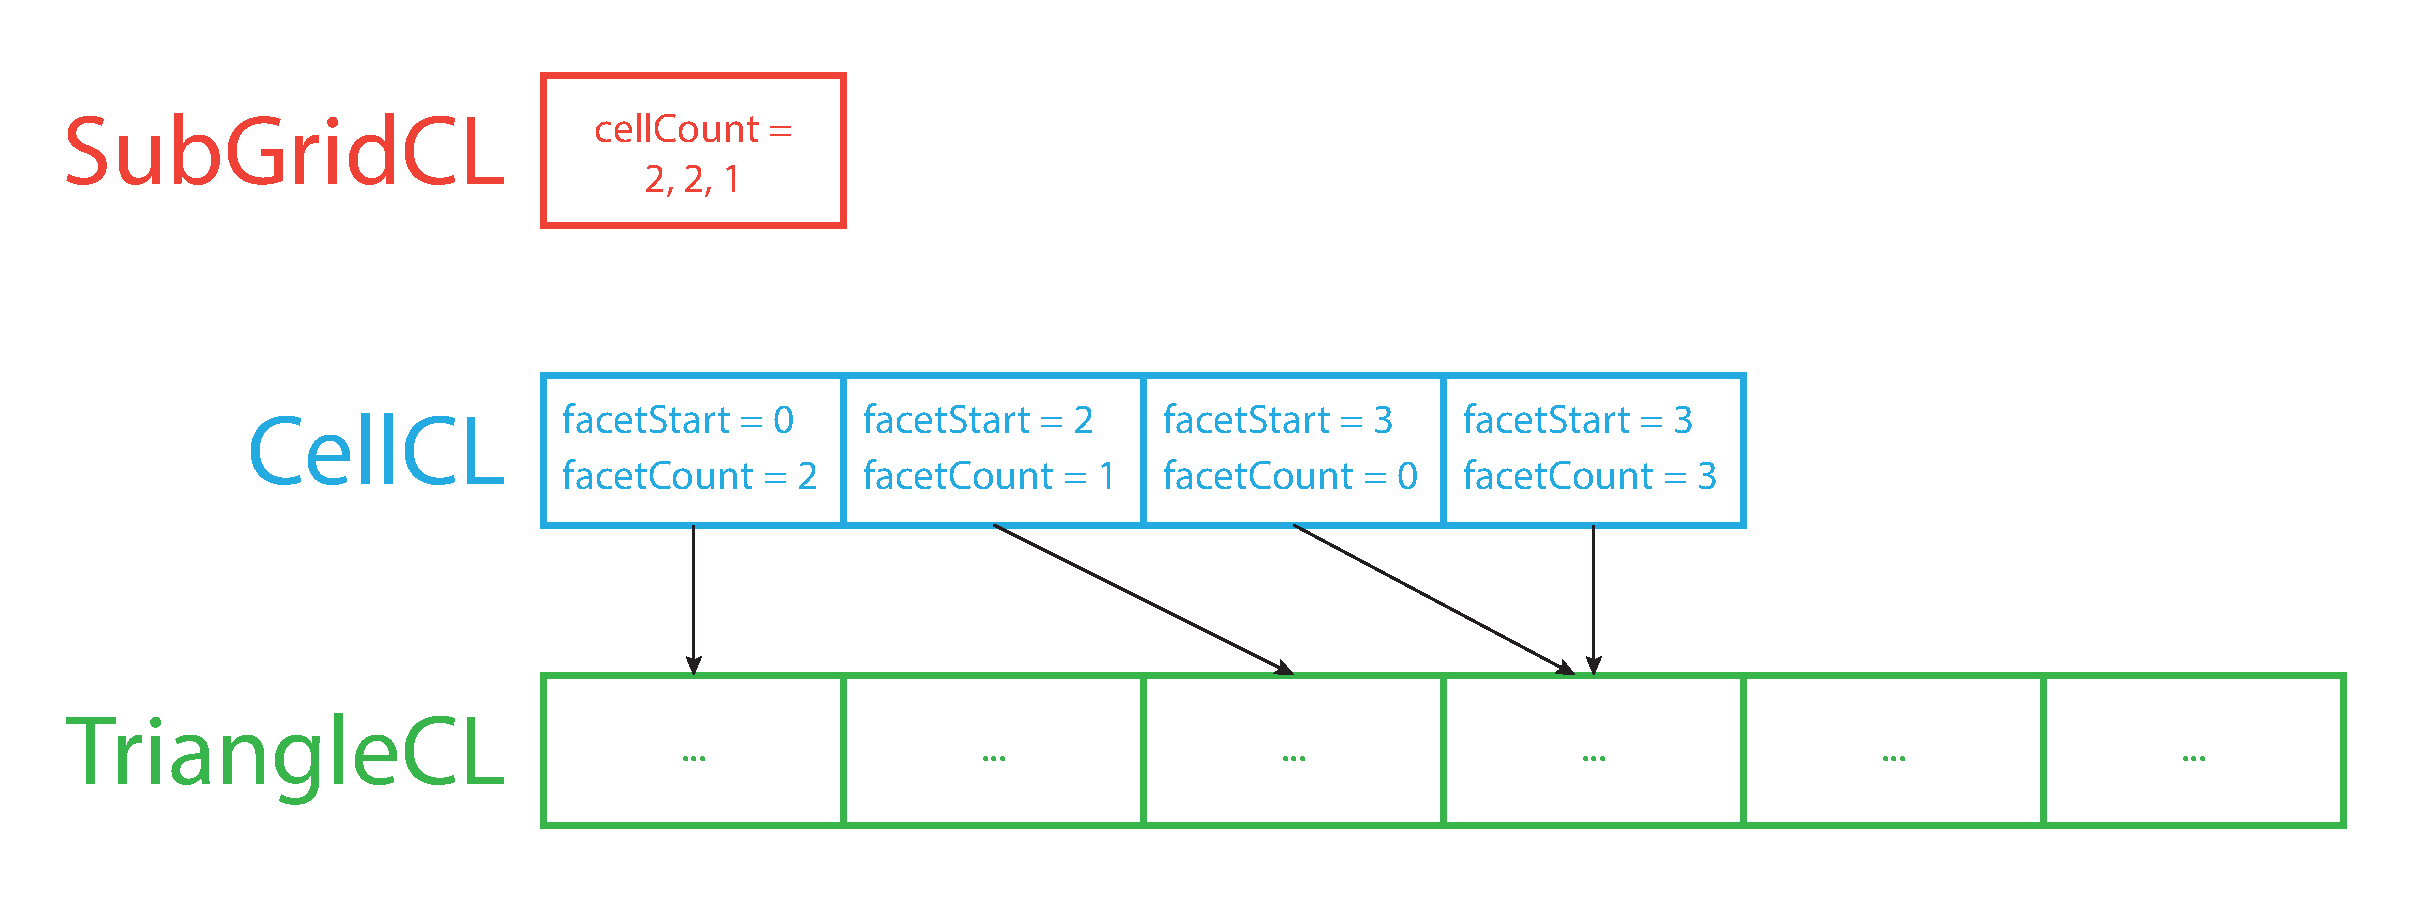
\includegraphics[width=0.8\textwidth]{buffer_layout}
\caption{Layout of the OpenCL buffers used to store the flattened grid.}
\label{fig:buffer_layout}
\end{figure}

Three buffers are required to store the grid. The first on is rather small and only stores meta information about the grid. It contains a single instance of the \lstinline!SubGridCL! struct which contains the \lstinline!cellCount! member. This cell count holds the extents of the grid in all three dimensions and therefore determines the number of cells.
The second buffer stores the cells as a large array of \lstinline!\CellCL! structures. Each of them may have multiple facets associated with them. Therefore, each cell has a \lstinline!facetStart! index which points to the first of \lstinline!facetCount! triangle belonging to this cell in the triangle buffer.
The third buffer then holds a huge array of triangles which contain the geometric information about the scene.

Flattening the grid into these three buffers has to be done every time a surface cell changes (e.g. by loading a new subtraction volume). When an update of the grid has occurred, the main application calls the \lstinline!OpenCLCasterWrapper!s \lstinline!update! method and passes the reference to the new grid. The grid is then flattened by the \lstinline!SubGrid! class, filling its members \lstinline!subGrid!, \lstinline!cells! and \lstinline!triangles!, which are exactly the contents of the three required OpenCL buffers. The \lstinline!SubGrid! instance is then passed to the currently loaded caster by calling the \lstinline!updateGrid! method. This method is implemented in \lstinline!AbstractCLCaster! and creates the actual OpenCL buffer objects and transfers the content of the \lstinline!SubGrid! to the GPU.

The kernel itself is again enqueued with a two-dimensional global work size of the size of the output image (one work item per pixel) rounded up to a multiple of the configured work group size. The kernel code for this first full ray casting approach starts equally as the TestCameraCaster. Each work item initially determines its ray direction. Then, the grid has to be traversed using the adapted 3D DDA algorithm based on John Amanatides and Andrew Woo presented in chapter \ref{sec:regular_grids} \cite{3DDDA}. This algorithm basically works by calculating the entry point of the ray into the grid as well as the corresponding cell of this entry point. Then, increment values for each dimension are calculated which are used to determine the next cell from the current one (details can be found corresponding paper). The collection of routines implementing this algorithm will be called cell traverser. After initialization, the ray casting kernel polls cells from this cell traverser until an intersection has been found or the grid has been fully traversed. For each cell returned by the cell traverser, all triangles inside this cell (determined by the \lstinline!facetStart! and \lstinline!facetCount! members)) are loaded from the triangle buffer and intersected using the same routine as in the TestCameraCaster. The intersection with the smallest distance to the ray origin (camera position) is selected as triangles are stored with no particular order guaranteeing depth sorted iteration. Cells however are returned in correct order by the cell traverser. Therefore, the traversal can be aborted if an intersection has been found inside a cell. The colorization of the output pixel is done equally to the TestCameraCaster by taking the dot product between the ray direction and the hit surface's normal.

The output of the SingleRayCaster is shown in figure \ref{fig:single}. Although the generated image is far from being a correct visualization, one can clearly recognize the shape of the cylinder head used as ray casting input (cf. the existing CPU caster result in figure \ref{fig:cylinder_head}).

\begin{figure}
\centering
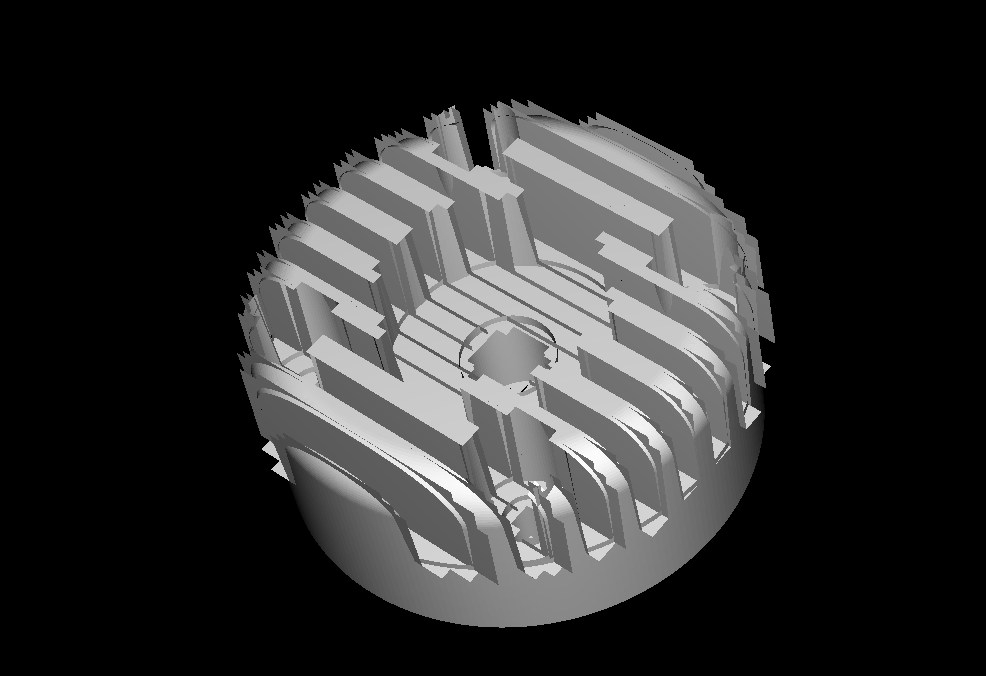
\includegraphics[width=0.5\textwidth]{single}
\caption{Screenshot of the OpenCL kernel output of the SingleRayCaster. The fringes sticking out of the cylinder head (especially visible at the top left) are due to hits on triangles of the subtraction volumes as the nearest triangle hit (regardless of which volume) is taken for the pixel's color. These errors will disappear when cell based counting is implemented.}
\label{fig:single}
\end{figure}


\subsection{SingleBooleanRayCaster}
\label{sec:single_boolean}

The SingleBooleanRayCaster extends the previous SingleRayCaster by using a counter for each ray which counts the number of volume entries and exits. The counting is done along the full traversal as discussed in chapter \ref{sec:boolean_raycasting}. As parts of the geometry are missing because of the classification of the grid (only the triangles of surface cells are stored in the grid and transfered to the GPU), this caster will probably produce erroneous results. However, this implementation would work if the complete geometry was present in the grid. This caster can be seen as an evolutionary step between the already presented SingleRayCaster and the SingleBooleanCellRayCaster, which will be able to handle open geometries.

The SingleBooleanRayCaster class is equal to the one of the previous SingleRayCaster. Also the kernel code starts off equally by calculating the ray direction for each work item/pixel and traversing this ray through the grid. Besides declaring the counter and initializing it with minus one, the only code that has changed it is the intersection routine of the ray with a cell polled by the cell traverser. The code still has to iterate over all triangles inside the cell and intersect the ray with each of them. However, instead of keeping the nearest intersection to the ray origin so far, we have to intermediately store all intersections of the ray with any triangle inside the cell. And here we hit a big problem in GPGPU computing with OpenCL, the lack of dynamic allocation.

Every kind of memory which is needed during a kernel execution has to be allocated beforehand. This accounts for both, global and local memory. Registers are handled a bit differently. Before a new work group is scheduled for execution on a streaming multiprocessor, all required registers for all work items of the work group have to be allocated in the register block on the SM. The number of registers required for a work item must therefore be determined in advance by the compiler (for all possible branches of the program, including all local variables) and is a decisive factor for how many work groups may be concurrently executed on a SM.

Let's consider the available options by an example. We take a common, small screen resolution of $1024 \times 768$ pixels. For each pixel a ray is created which needs a separate intersection buffer. As we do not know in advance how many intersections may maximally occur inside a cell, we have to define an allowed maximum. Let's say this value is a hundred (we actually had a long discussion about this in the office and thought about an even higher value, but a hundred proved to be sufficient in all used test scenes). Finally, we have to determine the size of the information required to hold an intermediate intersection for further processing. This must be at least the index of the hit facet (an unsigned integer), the distance of the intersection point from the ray's origin (a floating point value) and a boolean value (padded to four bytes) whether the ray enters the volume of the hit triangle or not. Details about the chosen information follow shortly. These three values make up twelve bytes. Let's calculate the total amount of memory required to hold a hundred intermediate intersection results per work item: $1024 * 768 * 100 * 12 = 943718400 B = 900 MiB$, which is a huge amount of memory for a GPU just for storing temporary data of an algorithm. Furthermore, this value does not include the actual processed data, the grid with its cells and triangles. Consequently, storing the intermediate intersections in global memory is not acceptable. \\
Using local (shared) memory for storing the intermediate intersections per work item would also be possible. However, local memory is quite small with sizes of 16, 32 or 48 KiB per SM. As each work item requires 1.2 KiB ($12 * 100$) the largest local memory configuration would only allow 40 work items to run concurrently on a SM which is an extremely poor occupancy considering the high amount of potentially concurrently executed threads per SM (e.g. 2048 on a NVIDIA Kepler GPU \cite[p.7]{kepler_arch}). \\
The third option is using registers. Although 1.2 KiB per work item do not fit most GPU's hardware limits (NVIDIA Kepler limits a thread to 63 (GK104) or 255 (GK110) 32 bit registers \cite{kepler_arch}), the kernel can still be launched. This shortage of registers is handled by compiler and driver by spilling the not available memory into global memory. As global memory is far slower accessed, register spilling usually causes a loss in performance. However, as the spilled area is rather small (several tens or hundreds of kilobytes) and the area is always accessed by the same SM, this part of global memory benefits strongly from the L1 cache on the SM and may still achieve good performance on reads and writes (Paulius Micikevicius from NVIDIA held a detailed presentation about this subject in CUDA \cite{register_spilling}).

As a result of this small analysis, it has been determined that the intersection buffer will be kept as local array inside the kernel. It is then up to the compiler to try to fit the array into registers or spill it into global memory. This buffer is then used to store all intersections of the ray with triangles inside the current cell. Afterwards, the intersections inside the buffer have to be sorted according to their distance to the ray's origin as the counter has to be altered in the same order as the ray hits the triangles. OpenCL does not provide a sorting routine of any kind. Thus, a sorting algorithm has to be implemented. As the maximum size of the intersection buffer is defined as a hundred, a simple insertion sort will be used as it performs well on small arrays and has very little overhead considering additional variables. After the buffer has been sorted, all intersections are iterated again (this time in the order they ray hits them) and the counter is incremented or decremented according to the hit triangles facing. If the counter reaches the value zero, the surface triangle has been found. The triangle id of the intermediately stored intersection is used to resolve the full triangle (with normal) and recalculate the exact intersection position. This information is then used to calculate the color value of the output pixel.

\begin{figure}
\centering
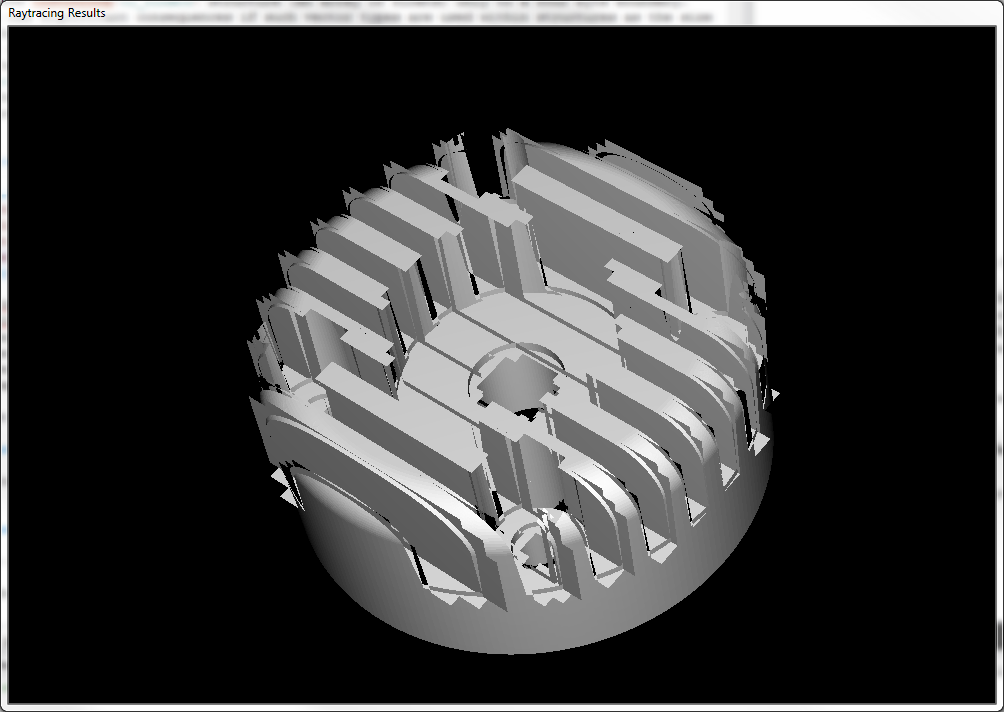
\includegraphics[width=0.5\textwidth]{singleboolean}
\caption{Screenshot of the OpenCL kernel output of the SingleBooleanRayCaster.}
\label{fig:singleboolean}
\end{figure}

The output of the SingleBooleanRayCaster is shown in figure \ref{fig:singleboolean}. The image does not look much better than the one of the SingleRayCaster and is still incorrect as the grid contains open geometries leading to invalid counting. However, by implementing counting an important step towards a working implementation has been made.

\subsection{SingleBooleanCellRayCaster}
\label{sec:single_boolean_cell}

The SingleBooleanCellRayCaster takes the previously described SingleBooleanRayCaster from chapter \ref{sec:single_boolean} and moves the counter initialization from before the cell traversal into the cell itself as explained in chapter \ref{sec:adapted_ray_casting}. The main unknown is thus the number of subtraction volumes the ray (in particular its entry point) is inside of at its cell entry. We have therefore to decide for each subtraction volume if the entry point lies inside the volume or not. A simple solution is to take any triangle of a subtraction volume and create a vector (secondary ray) from the entry point to a point on this triangle, which has to lie inside the current cell. According to the enclosed angle of the triangle's normal and the created secondary ray, it can be decided if the entry point is inside or outside of the subtraction volume the triangle belongs to. However, as multiple triangles of the same volume may be potentially hit by the secondary ray, it has to be ensured, that the secondary ray is not intersected by another triangle of the same volume (this case can lead to wrong decisions, as e.g. the secondary ray may select a triangle of the back size of volume and also intersect the front). The resulting initial counter value is initialized with zero and decremented for each subtraction volume the entry point is inside off.

The concrete implementation of this approach makes use of additional data provided in the \lstinline!TriangleCL! structure and is further based on an assumption guaranteed by the grid creation code of the main application. The \lstinline!clippedCentroid! member of the triangle structure (cf. class diagram in figure \ref{fig:enlight_opencl_class_diagram}) contains the centroid of the resulted polygon after the corresponding triangle has been clipped to its cell's bounding box. This value is calculated by the \lstinline!SubGrid! class when the grid of the main application is flattened into the OpenCL buffers. Furthermore, each triangle has a \lstinline!structureId! member which is an identifier being equal among all triangles inside a cell belonging to the same subtraction volume (structure). It is additionally guaranteed, that triangles belonging to the same structure are stored continuously in the triangle buffer. Based on these circumstances the counter initialization algorithm is implemented as follows.

Inside each work item, for each cell returned by the cell traverser, all triangles of the cell are iterated. Additional variables keep track of the current structure id, the current distance to the nearest triangle of the current structure and its normal. In each loop where the structure changes, a secondary ray is created from the primary ray's entry to clipped centroid of the current triangle of the loop which has caused the structure change. The distance from the entry point to the clipped centroid as well as this triangle's normal is kept. All following triangles (of the same structure) are then intersected with the created secondary ray. In case of an intersection, the distance to the nearest intersection of the secondary ray is updated as well as the normal by the one of the new, intersected triangle. Before the next structure change, the normal of the nearest triangle intersecting the created secondary ray can be used to determine if the entry point lies inside or outside of the current structure. If it is inside, the counter is decremented. The triangle iterating continues with the next structure analogously. After all triangles of the cell have been iterated, the initial counter value holds the number of subtraction volumes the primary ray's entry point is inside of. The algorithm can now continue equally as the SingleBooleanRayCaster by intersecting all triangles, sorting them by their depth and processing the counter along the ray to find the surface hit.

The SingleBooleanCellRayCaster is the first ray casting approach able to deliver correct results. The output image of the kernel is shown in figure \ref{fig:singlebooleancell}. Apart from a few wrong pixels which occur because of numeric instability of the used float data type (the do not occur on the CPU caster which uses double), the result already makes a satisfying impression. Considering the code however, there is still room for improvement as the kernel iterates all triangles of the cell twice. One time to determine the inside counter and one time for the intersections. Furthermore, the few invalid pixels may be eliminated if double precision would be used for the intersection routines on the GPU too. These two subjects will be addressed in subsequent chapters.

\begin{figure}
\centering
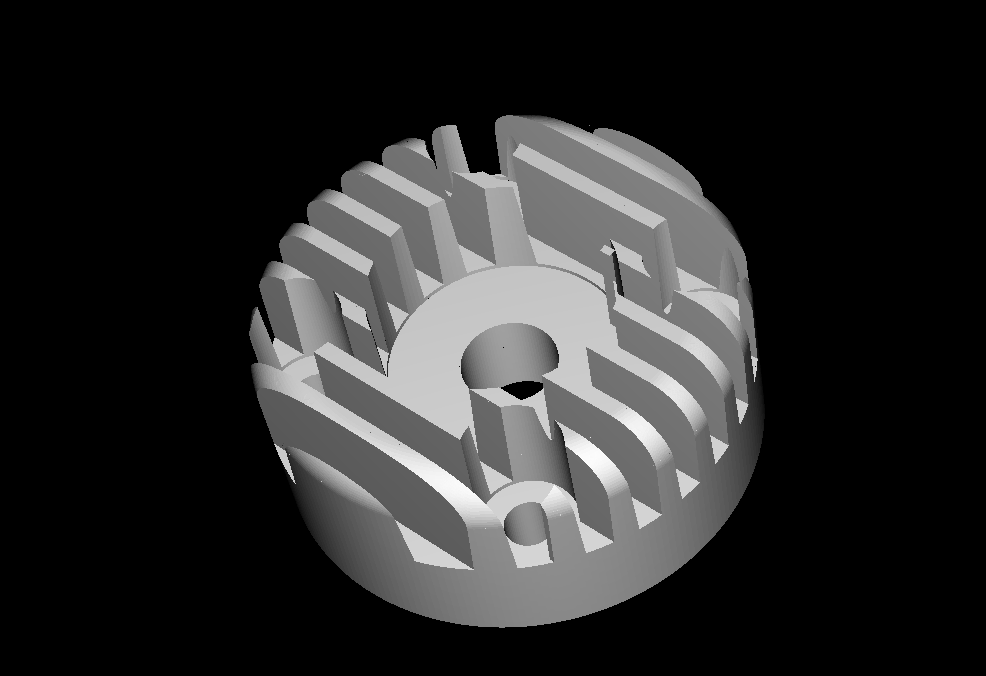
\includegraphics[width=0.5\textwidth]{singlebooleancell}
\caption{Screenshot of the OpenCL kernel output of the SingleBooleanCellRayCaster.}
\label{fig:singlebooleancell}
\end{figure}

\subsection{Double support in calculations}

Although the \lstinline!double! data type is very commonly seen in conventional languages like C++, Java or C\#, only recent GPUs support double precision floating point arithmetic. The reason for this is that the higher precision on the cost of speed did not fit the initial requirements of a graphics processing unit, which was optimized for maximum throughput. With the gaining popularity of GPGPU computing, hardware vendors also integrate double precision support within their hardware (e.g. the NVIDIA Kepler architecture provides special double precision units in addition to their normal cores \cite[p.8]{kepler_arch}). Some sensitive values of the \lstinline!RayCreationParameters! make already use of double precision types, as the program is expected to be run on newer hardware. However, most of the calculations inside the kernel are done using simple floating point arithmetic.

The anticipated benefit of using double precision for grid traversal and intersection routines is to reduce the number of erroneous pixels. These pixels are most often the result of rays which shoot between adjacent triangles or angles between secondary rays and normals of almost exactly 90$^\circ$ (where the dot product is a tiny positive or negative number). As OpenCL 1.2 is still very close to C99, no language features exist which would allow writing generic kernels. AMD has already proposed their OpenCL C++ static kernel language for standardization which would allow the use of classes, inheritance and especially templates, but it is not yet officially part of OpenCL and currently only supported on AMD systems. Therefore, the preprocessor will be used together with a compiler argument (when compiling the kernel at run time) to set the desired type. All floating point types involved in calculations inside the OpenCL code will be replaced by a corresponding token (e.g. \lstinline!T!, which is common in C++ templates) and defined when the OpenCL compiler is invoked (e.g. \lstinline! -DT=double!). Furthermore, also derived types must be defined to allow switching vector types (e.g. \lstinline!T3! for \lstinline!double3!).

This approach works well in practice. By recompiling the OpenCL kernel at run time, the used precision can even be changed on the fly without having to relaunch the main application. A corresponding console command has been implemented.

The SingleBooleanCellRayCaster with double precision already gets grid of most wrong pixels. However, the runtime of the kernel increased to over twice the amount of the single precision variant.

To also support older GPUs without double precision an additional preprocessor option was introduced (also affecting the main C++ application) which allows forcing the floating point precision to single. This also overrides the double values of the transfer structures.

\subsection{OpenCL source embedding}

One of the big strengths of OpenCL is its portability across many different hardware platforms. This big advantage is achieved by delaying the compilation of the OpenCL source code until an application's actual execution on the target platform. However, this concept usually forces programmers which put their OpenCL code in dedicated files to ship parts of their source code with the compiled application. This scenario is undesired or even prohibited in commercial software development where the customer should not gain access to a product's source code. Furthermore, keeping the OpenCL source files in the correct place for the application to find them at run time requires additional deployment overhead. Fortunately, both problems can be solved by embedding (and optionally even encrypting) the OpenCL source code into the actual program. Although several easy solutions exist on different operating systems or technologies (e.g. resource files on windows), no cross platform or C++ standard compliant method for storing an applications resources is available.

However, an OpenCL source file basically contains text and text can be statically stored inside an application using a string literal (which is an array of characters). It is therefore possible to store the required OpenCL code inside a large character array which is compiled into the executable. Fortunately, the corresponding OpenCL API call for creating an OpenCL program from source does not take the name of a file as argument but the actual source code. Therefore, the embedded character array can be directly passed to OpenCL.

Nevertheless, editing source code in a separate file is more comfortable for the programmer and better handled by IDEs concerning syntax highlighting and debugging than writing OpenCL code directly as string literals into the existing C++ code. Therefore, a separate conversion tool has been developed which reads in a given input file and outputs a C++ header file with a character array containing the content of the input file. This header can than be included and used by the existing C++ application. Modern build systems (like MSBuild and Visual Studio) also support the configuration of custom build steps, which allows the creation of includable headers from the OpenCL source files as part of the build process in Visual Studio. Visual Studio therefore calls the external conversion tool for every OpenCL source file which is part of the project before it starts compiling the C++ files.

This solution works for simple OpenCL source files. However, the preprocessor's \lstinline!#include! directive allows an OpenCL source file to include other source files. If an OpenCL source code containing includes would be embedded directly, the application would fail to include the referenced files at run time after deployment. Therefore, a little bit more logic has to be added to the external conversion tool. Specifically, the OpenCL source code has to be scanned for \lstinline!#include! directives and they have to be recursively resolved (included files can include further files) before the text can be converted into the output character array. Furthermore, as this process drops the original file names and line numbers, proper \lstinline!#line! macros have to inserted to allow the compiler to report errors on their correct origin. Although this is basically a small implementation of a part of a preprocessor, an existing preprocessor (like Microsoft's one) could not be used as conditional compilation should still be possible after the conversion (e.g. to define a macro when invoking the OpenCL compiler which is checked by an \lstinline!#ifdef! directive).


\subsection{SinglePrimaryBooleanCellRayCaster}
\label{sec:single_primary}

The last single ray caster implementation takes the previous one, the SingleBooleanCellRayCaster from chapter \ref{sec:single_boolean_cell}, and merges the two loops which iterate over the triangles of the current cell into one. Furthermore, secondary rays are only cast when the primary ray does not hit a structure.

The host code for this caster implementation is exactly the same as of the SingleBooleanCellRayCaster. The kernel starts equally by computing the ray direction and starting the grid traversal using the cell traverser. For each cell the initial counter value has to be calculated as well as all intersections. These two steps were executed after each other in the previous implementation and are merged now. Before iterating over the triangles of the current cell, the intersection buffer is declared together with a variable holding the current structure id, the start triangle index of the current structure as well as normal and distance to the nearest intersection of the current structure. Then, the algorithm starts to poll the triangles of the current cell from global memory. The \lstinline!structureId! member is again monitored inside the loop over the triangles. On a structure change (and on the first loop iteration), we save the index of the current triangle as start index of the new structure. During the triangles of this structure the primary ray is intersected with each triangle. If an intersection is found, the intersection is added to the intersection buffer and the distance from the primary ray's origin to the intersection point as well as the hit triangle's normal vector is stored. Before the next structure change (after the last triangle of a structure), the algorithm checks if the primary ray has intersected a triangle of the current structure. If this is the case we can determine if the entry point lies inside the current structure by using the normal vector of the hit triangle and the primary ray's direction. If the primary ray did not hit any triangle of the structure, we have to use secondary rays. In this case, the triangles of the current structure are iterated again (we have stored the start triangle index on each structure change for this reason). A secondary ray is created to the clipped centroid of the first triangle and all subsequent triangles of the same structure are intersected with the secondary ray. The nearest hit of the secondary ray is then used to determine if the primary ray is inside this structure or not (equally as in the previous implementation for all structures). After all triangles have been iterated, we have the buffer of intersections as well as the initial inside counter value and can continue with depth sorting the intersections and processing the counter along them to find the surface hit.

This approach has two advantages over the previous one. Firstly, each triangle of a cell is only requested once from global memory instead of two times which should improve performance. Secondly, using the primary ray for determining if the entry is inside a volume or not produces more stable results as many of the erroneous pixels have been disappeared. This is the final single ray casting variant which is also used as the main application's default ray casting routine. The output of the ray caster is shown in figure \ref{fig:singleprimary}.

Further optimization of this implementation is surely possible but would require the help of advanced tools like a GPU profiler. However, NVIDIA dropped OpenCL support with CUDA Toolkit 5.0 (not officially announced but the topic is discussed in several internet forums \cite{dropped_opencl_support}), which was used during the internship.


\begin{figure}
\centering
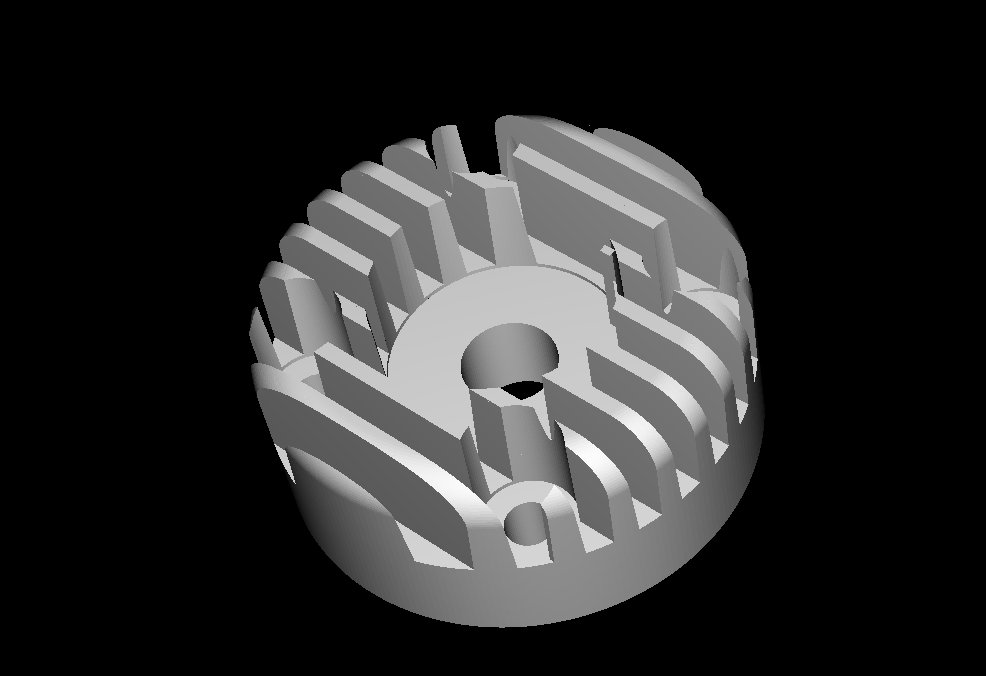
\includegraphics[width=0.5\textwidth]{singleprimary}
\caption{Screenshot of the OpenCL kernel output of the SinglePrimaryBooleanCellRayCaster.}
\label{fig:singleprimary}
\end{figure}

\subsection{PacketRayCaster}

The PacketRayCaster approaches differently than the single ray variants and is primarily motivated by the huge performance boost achieved by the CPU implementation compared with the previous single ray CPU version. The general performance consideration is to keep a group of adjacent rays as coherent as possible to benefit from better vectorization and caching behavior. Furthermore, traversing whole packages instead of each single ray reduces the overall control logic.

Although the PacketRayCaster shares some code with the final SinglePrimaryBooleanCellRayCaster, a lot of changes are necessary to the kernel code. Fortunately, the host code does only require a little adjustment, which is to define a packet width and height which is used as the kernels local work size. The remaining host code stays the same, meaning the kernel is again enqueued using a two-dimensional range with the size of the output image where each dimension is rounded up to the next multiple of the defined packet width or height.

The kernel code then begins again by determining the ray direction for each work item using the \lstinline!RayCreationParameters!. Afterwards, the four corner rays are marked by declaring an integer for each work item which is initialized to minus one and only set to a valid index (from zero to three) by the four work items in the corners of the work group, identified using their local ids. This integer can then be easily used to detect if the current work item is a corner ray or not. Furthermore, the four corner ray work items write their ray directions into a shared array in \lstinline!__local! memory. \\
Now the traverser algorithm can be set up. The packets will be navigated through the grid slice by slice as described in chapter \ref{sec:packet_casting}. However, a traversal is only necessary if the ray packet actually hits the grid. This check is performed by trying to intersect the outer square of rays of the packet (called peripheral rays) with the bounding box of the grid. If any of them hits, a traversal is necessary. Therefore, a main traversal axis has to be determined which is done by selecting the axis where the corresponding component of the central ray's direction vector has the largest magnitude. All corner rays are then intersected with the front plane of the first slice of the grid. The main traversal axis as well as the front plane intersection points are stored in local memory. The slice traverser is now initialized. \\
The kernel then continues with the traversal loop, which polls cells from the slice traverser. The slice traverser keeps state information about the current slice and the current cell's coordinates inside the current slice. Initially, when the first cell is requested, the slice traverser intersects the four corner rays with the black plane of the current first slice. Using the maximum and minimum values of the intersection points on the front and back plane of the slice of the non-traversal axes, the rectangle on the slice which has been hit by the packet can be determined. This rectangle is extended to full cell boundaries and the slice traverser can return the first cell of this range. Subsequent cell requests can be satisfied returning further cells of this range until all cells of the hit slice region have been iterated. Then the slice traverser has to move on to the next slice by intersecting the corner rays with the back plane of the next slice Using the intersection points of the last slice's back plane as intersection points of the now current slice's front plane, the affected cell region can again be determined. This process is repeated until all cells of the last slice have been returned or the traversal is aborted. \\
For each cell returned by the slice traverser, the packet has to be intersected with the triangles inside the cell. However, before all rays inside the packet are intersected with all triangles, several optimizations are done. Each corner ray work item creates a plane using the next clockwisely adjacent corner ray direction from shared memory. The result are four planes bounding the frustum of the ray packet which allows culling of the cell's triangles against it. However, this frustum culling step can only be done by one thread of the packet which has to actually hit the cell (a cell hit by the ray packet does not necessarily need to be hit by all rays of the packet). \\
The culling is done by iterating over all triangles of the current cell. Each triangle's vertices are then checked against all frustum planes. If all vertices lie outside of one plane, the triangle is culled. This approach does not cull all possible triangles but it is fast and easy to implement as it does not require any intersection tests. The indexes of all triangles which are not culled are accumulated in a buffer in local memory, and therefore visible to all work items afterwards. However, the culling routine has to keep an eye on the centroids of the unculled triangles. As triangles of a structure lying outside the packet's frustum are culled, a secondary ray targeting a centroid outside the frustum of an unculled triangle may lead to wrong results, as a potentially, with the secondary ray intersecting triangle was removed during culling. Therefore, the culling routine has to ensure, that the first triangle of each structure provides a valid centroid lying inside the packets frustum.
A further optimization is also possible during the culling routine. By also monitoring the structure changes we can determine the case in which all triangles of a structure are culled. If this is the case, a secondary ray can be used to determine if the frustum lies inside this culled structure which allows to skip the current cell entirely. \\
After the culling step completed, a barrier operation is executed to ensure that the culling thread has finished writing the indexes of the unculled triangles into local memory before any work item starts to read them. After this synchronization point, each work item can then proceed with the intersection routine taking the array of unculled triangle indexes in shared memory. The intersection is done equally as in the SinglePrimaryBooleanCellRayCaster, by iterating all triangles and intermediately storing the intersections in a buffer. The initial value of the inside counter is also determined in this step. Secondary rays are used if the primary ray does not intersect a subtraction volume. The intersections are then sorted again and the counter is processed along them to find the surface hit.

Although the packet ray caster produces visually equivalent results as the SinglePrimaryBooleanCellRayCaster (cf. Figure \ref{fig:packet}), it is despite the optimizations slower than the single ray variant. The reasons are probably the large amount of synchronization points (barriers) encountered during the kernel execution, which are needed every time a shared state is written, which happens a lot inside the slice traverser. However, a detailed analysis requires the use of professional tools like profilers, which were not used during the internship (cf. end of chapter \ref{sec:single_primary} for the reason). Another, yet unsolved problem is that the packet ray caster crashes occasionally, especially when enqueued multiple times with short delay or when being compiled with double precision.


\begin{figure}
\centering
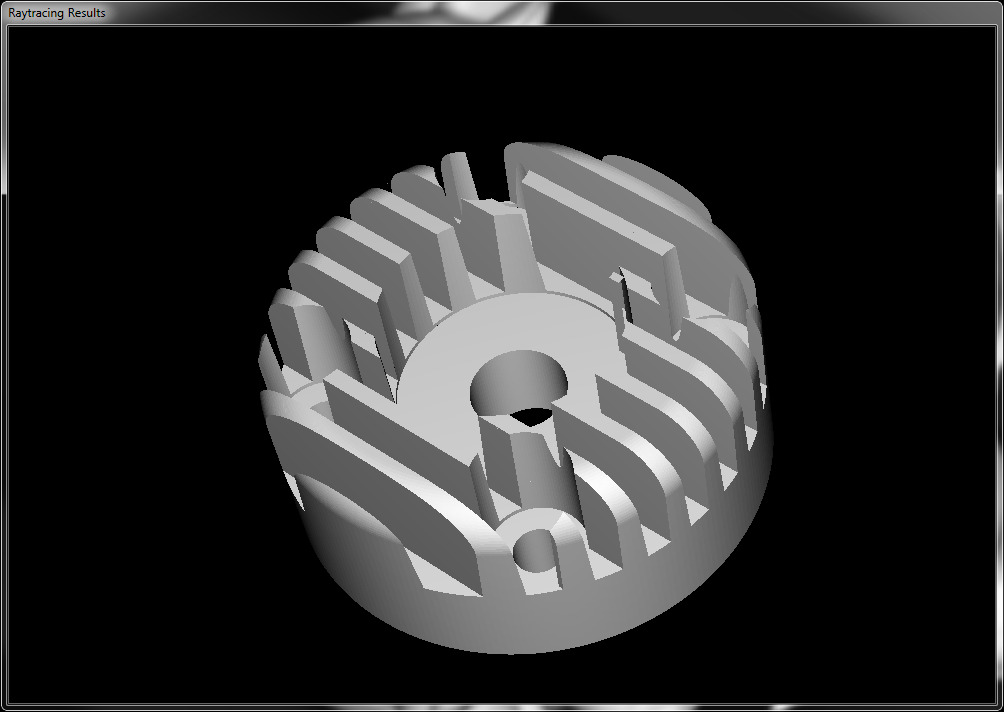
\includegraphics[width=0.5\textwidth]{packet}
\caption{Screenshot of the OpenCL kernel output of the PacketRayCaster.}
\label{fig:packet}
\end{figure}

\subsection{Migration to new host application}
\label{sec:migration}

While the main development of Enlight happened using the code base of an existing, RISC internal framework designed for easy OpenGL integration and scene management, Michael Hava, one of the project members, was already working on a newer, leaner main application which would then also be used for the final product. The main design consideration of this new application was to get rid of legacy code (like the OpenGL framework and MFC) and to separate the application into components using a self-written C++ component framework by Michael Hava called CWC. Furthermore, by using the cross-platform GLFW library for window management and user interaction, the application may be run on all major platforms.

Although the complete main application was rewritten, the final port of the OpenCL caster suite to this new prototype did only require an adaption of the \lstinline!OpenCLCasterWrapper! class. Of main concern were the \lstinline!RegularGrid! class and the \lstinline!PixelGrid! class, which where both replaced by other structures. Updates to the OpenCL driver now occur separately for each cell and may be executed concurrently by multiple threads. Therefore, thread safety of the \lstinline!OpenCLCasterWrapper!'s methods had to be ensured which was implemented using C++11's new thread library. Furthermore, the concept of configurable driver options was generalized to key value pairs settable by the main application. Examples of the OpenCL caster include floating point precision, currently used caster implementation, work group size, OpenCL platform or device and out of core casting. The final and largest change was also the output format of the casters, which was changed from an image with red, green, blue and depth channel to the hit triangle id and distance as well as the barycentric coordinates of the intersection point on the triangle. The actual color image is then calculated by the main application, separating the shading step from the ray casting algorithms.


\subsection{Out-of-core ray casting}
\label{sec:out_of_core}

The final implemented feature is optional out-of-core ray casting which affects all ray casters. The basic concept of out-of-core algorithms is to allow the processing of data structures which are larger than the available system memory. Concerning the GPU ray casting implementation, scenes should be supported where the grid representation is larger than the available memory on the graphics card. The available main memory is still a limit for the scene's size.

When designing an out-of-core approach for the grid based GPU ray casters, we are limited by the design of OpenCL. OpenCL requires, that all global memory objects (like the three buffers where the grid, cells and triangles are stored) have to be created and fully initialized before a kernel is executed. Furthermore, these objects cannot be changed during the execution of a kernel. Additionally, communication between the host application and a running kernel is one-way. No way exists for a kernel to communicate back to the host application. These constraints limit the design of an out-of-core caster as such, that all required information for a kernel have to be set up before the kernel is enqueued and the kernel cannot request further data during it's execution. Therefore, the grid has to be divided into smaller sub grids which have to be ray casted individually and merged into a final output image. Fortunately, dividing the grid causes no problems as the ray casting algorithms already operate on a cell basis. Also, merging the output images should inflict no problems, as every pixel contains depth information.

Out of core casting can be enabled on the console of the main application and an optional out of core buffer size may be specified (e.g. for testing purposes). If this value is not specified, it is set to the maximum available buffer size. When the main application passes the grid to the \lstinline!OpenCLCasterWrapper!  by calling the \lstinline!update! method, the wrapper checks if out of core casting is enabled. If this is the case, it passes the grid to the static \lstinline!SubGrid::divideGrid! method, which recursively splits the grid in half, changing the split axis on each recursion, until each sub grid requires fewer memory than the current out of core buffer size. These sub grids are then flattened and stored in the \lstinline!subGrids! member of the wrapper.

When the scene should be ray casted, the sub grids are depth sorted depending on the current camera position. A loop than iterates over the sub grids starting at the nearest. The sub grid is transfered to the GPU and ray casted. Each work item of a subsequent ray cast (the second to the last one) then checks the buffer containing the output image if the corresponding pixel has already been written to. If this is the case, the work item can exit. This approach ensures that no pixels are ray casted twice. Therefore, apart from the memory transfers of the sub grids which have to be done for every ray casted image, no additional overhead is produced. 
